% 04_line_of_sight.tex
\section{The line-of-sight integral}
\label{ch:los}

In principle the Boltzmann hierarchy of chapter 3 gives us the photon distribution $\Theta_\ell(\vec k, \tau_0)$ at the observer for every $\ell$ and $\vec k$. In practice this is hopeless: to get to $\ell_\mathrm{max} \approx 2500$ we would need to evolve thousands of multipoles per mode, with each multipole receiving streaming power from below. The numerical cost is prohibitive.

Seljak and Zaldarriaga (1996) found a way out. Their observation is that the Boltzmann equation can be written in integral form, with the streaming part of the operator turned into a spherical Bessel function, leaving only the \emph{source terms} -- scattering, monopole, Doppler, ISW -- to be computed dynamically. Then we evolve the hierarchy only to the few low multipoles needed to build the sources (typically $\ell \leq 3$), and project them onto the sphere with a line-of-sight integral. This chapter derives that integral and constructs the source function.

\subsection{Spherical-harmonic toolbox}

The geometry of the projection from $\vec k$-space to the sky requires three identities. They are standard and we collect them here for reference.

\paragraph{Plane wave expansion.} A plane wave with wavevector $\vec k$ expanded in spherical harmonics about an origin:
\begin{equation}
  e^{i\vec k \cdot \vec x} = 4\pi \sum_{\ell m} i^\ell\, j_\ell(kr)\, Y^*_{\ell m}(\hat k)\, Y_{\ell m}(\hat x).
  \label{eq:plane_wave_exp}
\end{equation}
Equivalently, in the form we will use:
\begin{equation}
  e^{i\vec k \cdot \vec x} = \sum_\ell (2\ell + 1)\, i^\ell\, j_\ell(kr)\, P_\ell(\hat k \cdot \hat x).
\end{equation}

\paragraph{Spherical Bessel functions.} Defined by
\[
  j_\ell(x) = \sqrt{\frac{\pi}{2 x}}\, J_{\ell + 1/2}(x).
\]
For small argument $j_\ell(x) \sim x^\ell/(2\ell + 1)!!$; for large argument $j_\ell(x) \sim x^{-1}\sin(x - \ell\pi/2)$. Near $x = \ell$ there is a peak and the function transitions from exponentially suppressed to oscillatory. This sharp localisation in $k \cdot r$ near $\ell/r$ is what makes the Limber approximation (chapter 6) work and what allows us to localise transfer-function support in $k$.

The recurrence we will use repeatedly:
\begin{equation}
  j_\ell'(x) = \frac{\ell}{x}\, j_\ell(x) - j_{\ell + 1}(x),
  \qquad
  j_\ell''(x) = -\frac{2}{x}\, j_\ell'(x) + \Bigl(\frac{\ell(\ell+1)}{x^2} - 1\Bigr)\, j_\ell(x).
  \label{eq:jl_recurrence}
\end{equation}

\paragraph{Addition theorem.}
\[
  P_\ell(\hat k \cdot \hat n) = \frac{4\pi}{2\ell + 1}\sum_m Y_{\ell m}(\hat k)\, Y^*_{\ell m}(\hat n).
\]
This is how we move from the $\vec k$-axis frame (where the Boltzmann hierarchy lives) to the sky frame (where we project onto $Y_{\ell m}$ harmonics).

\subsection{From the Boltzmann hierarchy to an integral}

We work with the conformal time variable $\tau$ along a photon trajectory from last scattering to today. A photon arriving at the observer from direction $\hat n$ at time $\tau_0$ has, at the earlier time $\tau$, the spatial position $\vec x(\tau) = (\tau_0 - \tau)\,\hat n$. Write $\chi(\tau) = \tau_0 - \tau$ for the comoving distance back to that time.

The Boltzmann equation for the temperature anisotropy along a photon path is
\begin{equation}
  \frac{\mathrm{d}}{\mathrm{d}\tau}(\delta T/T) + \dot\kappa\,(\delta T/T) = S^T(\vec x, \hat n, \tau),
  \label{eq:Boltzmann_path}
\end{equation}
where the source $S^T$ collects all non-streaming terms: Thomson scattering off electrons (which feeds in $\Theta_0 + \mu v_b + \tfrac{1}{2}P_2(\mu)\Pi$ from the monopole, Doppler, and polarisation-quadrupole contributions), the gravitational redshift $\dot\Phi + \mu^2\dot h/2$ (the ISW + Sachs-Wolfe terms), and so on. The integrating factor for \cref{eq:Boltzmann_path} is $e^{-\kappa(\tau)}$, and integrating gives the formal solution
\begin{equation}
  (\delta T/T)(\hat n, \tau_0) = \int_0^{\tau_0} S^T(\vec x(\tau), \hat n, \tau)\, e^{-\kappa(\tau)}\,\mathrm{d}\tau.
  \label{eq:LOS_path}
\end{equation}
The factor $e^{-\kappa(\tau)}$ is the probability that a photon survived from $\tau$ to today without re-scattering. This is the line-of-sight form: an integral over conformal time of a source weighted by the surviving fraction.

\subsection{Going to $\vec k$-space and projecting onto multipoles}

Fourier transform \cref{eq:LOS_path}, expand $e^{i\vec k\cdot \vec x(\tau)} = e^{i k\chi(\tau)\,\mu}$ using \cref{eq:plane_wave_exp}, and project onto multipoles using the addition theorem. After lengthy but standard algebra the result is the line-of-sight integral for the temperature transfer function:
\begin{equation}
  \Delta^T_\ell(k) = \int_0^{\tau_0}\,\mathrm{d}\tau\,\bigl[\widetilde S^T_0\, j_\ell(k\chi) + \widetilde S^T_1\, j_\ell'(k\chi) + \widetilde S^T_2\, j_\ell''(k\chi)\bigr],
  \label{eq:Delta_T}
\end{equation}
with $\chi = \tau_0 - \tau$, and where the three source components are
\begin{align}
  \widetilde S^T_0 &= 2\, \dot\Psi_W\, e^{-\kappa} + g\,(\Theta_0 + \Psi_W + \tfrac{5}{8}\Pi), \\
  \widetilde S^T_1 &= g\,(\sigma + v_b), \\
  \widetilde S^T_2 &= \tfrac{15}{8}\, g\, \Pi.
\end{align}
Here $g(\tau) = \dot\kappa\,e^{-\kappa}$ is the visibility function from chapter 2, and $\Pi = (\pi_\gamma + 9 E_2/5)/10$ is the polarisation source. The three terms in $\widetilde S^T_0$ correspond to the integrated Sachs-Wolfe effect (ISW), the Sachs-Wolfe + intrinsic temperature contribution at last scattering, and a small quadrupolar contribution to the temperature monopole. The $\widetilde S^T_1$ piece is the Doppler effect: photons scatter off baryons whose peculiar velocity is $v_b$. The $\widetilde S^T_2$ piece is the quadrupole-induced polarisation feedback.

\paragraph{Why three Bessel channels?}
The original Seljak-Zaldarriaga source had a single Bessel function $j_\ell$ multiplied by a long expression. Integration by parts on the $\dot v_b$ and $\dot\Pi$ terms moves the time derivatives off the source and onto the kernel, generating $j_\ell'(k\chi)$ and $j_\ell''(k\chi)$. The boundary terms vanish because $g(\tau)$ is zero outside recombination/reionisation. The advantage is that $\widetilde S^T_0, \widetilde S^T_1, \widetilde S^T_2$ are all built from low-$\ell$ photon multipoles ($\Theta_0$, $\Theta_2$, $E_2$) plus metric variables; we do not need the full hierarchy.

\subsection{The $E$-mode source}

For polarisation a similar derivation, with spin-weighted spherical harmonics in place of ordinary $Y_{\ell m}$, gives
\begin{equation}
  \Delta^E_\ell(k) = \sqrt{(\ell + 2)!/(\ell - 2)!}\,\int_0^{\tau_0}\,\mathrm{d}\tau\,\widetilde S^E\, \frac{j_\ell(k\chi)}{(k\chi)^2},
  \label{eq:Delta_E}
\end{equation}
with the $E$-mode source
\begin{equation}
  \widetilde S^E = \frac{15}{8}\, g\, \Pi.
\end{equation}
The geometric prefactor $\sqrt{(\ell+2)!/(\ell-2)!} \approx \ell^2$ for large $\ell$ comes from the differential operator that turns the spin-2 polarisation field into the scalar $E$ mode. The $1/(k\chi)^2$ is the dual Bessel-function factor that makes \cref{eq:Delta_E} the correct projection of a spin-2 source.

\subsection{Source-function decomposition in the code}

To match the numerical structure of \cref{eq:Delta_T}, our code returns four arrays per $(k, \tau)$ pair:
\[
  \texttt{src\_j0} = \widetilde S^T_0,\qquad
  \texttt{src\_j1} = \widetilde S^T_1,\qquad
  \texttt{src\_j2} = \widetilde S^T_2,\qquad
  \texttt{src\_E} = \widetilde S^E\big/\bigl(\chi^2 k^2\bigr).
\]
The $1/(\chi^2 k^2)$ factor in \texttt{src\_E} absorbs the $1/(k\chi)^2$ in \cref{eq:Delta_E} ahead of time, so the LOS integral simply convolves \texttt{src\_E} with $j_\ell$ -- no separate Bessel-derivative book-keeping for the $E$ mode.

\subsection{Building the source function: gravitational potentials}

The synchronous-gauge code from chapter 3 carries $\eta$ and $h$, not $\Phi$ and $\Psi$. To use the line-of-sight formula we need to reconstruct the Newtonian-gauge metric variables, or equivalently the Weyl potential $\Psi_W$. The relation in synchronous gauge is
\begin{equation}
  \Psi_W = -\frac{1}{2 k^2}\bigl[(8\pi G a^2\delta\rho + 3 \mathcal{H} 8\pi G a^2 (\rho + p)\theta/k) + 8\pi G a^2 (\rho + p)\sigma_\text{anis}\bigr],
  \label{eq:Weyl}
\end{equation}
where the bracketed combination is the same one that enters the Einstein 00-equation. Its time derivative $\dot\Psi_W$, which sources the ISW effect, can be evaluated from the Boltzmann hierarchy without re-evaluating the full RHS -- we have all the ingredients ($\dot\pi_\gamma$, $\dot\pi_\nu$, $\dot\sigma$) already.

\subsection{The code: \texttt{build\_sources}}

\begin{codebox}[Cell: \texttt{build\_sources}]
\begin{lstlisting}[style=python]
def build_sources(tau, y, k, pgrid, thermo):
    """Source function building blocks at a single (k, tau) point.

    Returns (ISW, monopole, sigma+vb, vis, polter, source_E) -- the
    raw pieces that get combined into the three temperature Bessel
    channels and the E-mode source.
    """
    (a, adotoa, grhog_t, grhor_t, grhoc_t, grhob_t,
     dgrho, dgq, z, sigma,
     etak, clxc, clxb, vb, clxg, qg, pig, clxr, qr, pir) = _common_terms(
        tau, y, k, pgrid['bg_vec'], pgrid['sp_a_x'], pgrid['sp_a_c'])
    opacity = max(float(_cubic_eval(pgrid['sp_op_x'], pgrid['sp_op_c'], tau)),
                  1e-30)
    k2 = k * k

    E2 = y[IX_POL] if LMAXPOL >= 2 else 0.0

    # --- Weyl potential phi = (Phi + Psi)/2 in synchronous gauge ---
    dgpi = grhog_t * pig + grhor_t * pir
    phi  = -((dgrho + 3.0 * dgq * adotoa / k) + dgpi) / (2.0 * k2)

    # --- Compute phi_dot directly from hierarchy equations ---
    polter = pig / 10.0 + 9.0 / 15.0 * E2
    Theta3 = y[IX_G + 3] if LMAXG >= 3 else 0.0
    N3     = y[IX_R + 3] if LMAXNR >= 3 else 0.0
    pigdot = (2*k/5*qg - 3*k/5*Theta3 - opacity*(pig - polter) + 8*k*sigma/15)
    pirdot = (2*k/5*qr - 3*k/5*N3 + 8*k*sigma/15)
    pidot_sum  = grhog_t * pigdot + grhor_t * pirdot
    diff_rhopi = pidot_sum - 4.0 * adotoa * dgpi
    gpres_plus_grho = (4.0/3.0) * (grhog_t + grhor_t) + grhoc_t + grhob_t
    phidot = 0.5 * (adotoa * (-dgpi - 2.0 * k2 * phi) + dgq * k
                     - diff_rhopi + k * sigma * gpres_plus_grho) / k2

    # --- Visibility and exp(-tau) at this time ---
    tau_min, tau_max = thermo['tau_arr'][0], thermo['tau_arr'][-1]
    if tau < tau_min or tau > tau_max:
        vis    = 0.0
        exptau = np.exp(-thermo['tau_optical'][0]) if tau < tau_min else 1.0
    else:
        vis    = float(thermo['visibility_interp'](tau))
        exptau = float(thermo['exptau_interp'](tau))

    # --- Three source components ---
    ISW       = 2.0 * phidot * exptau                       # 2 phi_dot e^{-kappa}
    monopole  = -etak / k + 2.0 * phi + clxg / 4.0          # Theta_0 + Psi_W + (3/8) delta_b...
    chi       = pgrid['tau0'] - tau
    source_E  = 15.0 / 8.0 * vis * polter / (chi**2 * k2) if chi > 0 else 0.0

    return ISW, monopole, sigma + vb, vis, polter, source_E
\end{lstlisting}
\end{codebox}

\paragraph{Walking through the function.}
\begin{itemize}
  \item \texttt{phi} is the Weyl potential $\Psi_W$ computed from \cref{eq:Weyl}: the combination of $\delta\rho$, $(\rho + p)\theta$, and anisotropic stress that appears in the Einstein 00-equation.
  \item \texttt{phidot} is its time derivative, computed directly from the hierarchy equations -- this avoids re-evaluating the full Boltzmann RHS just to get $\dot{\Psi}_W$.
  \item \texttt{ISW = 2 phidot exptau} is the integrated Sachs-Wolfe contribution to $\widetilde S^T_0$.
  \item \texttt{monopole = -etak/k + 2 phi + clxg/4} is the Sachs-Wolfe combination $\Theta_0 + \Psi_W$ in synchronous gauge.
  \item \texttt{sigma + vb} is the Doppler source $\widetilde S^T_1$ apart from the visibility prefactor.
  \item \texttt{polter} is the polarisation source $\Pi = \pi_\gamma/10 + 9 E_2/15$.
  \item \texttt{source\_E} is $\widetilde S^E/(k\chi)^2 = (15/8)\, g\, \Pi/(k\chi)^2$, ready for the LOS integral.
\end{itemize}

The caller (\texttt{evolve\_k} in the next chapter) assembles these into the three temperature channels
\[
  \texttt{src\_j0} = \texttt{ISW} + \texttt{vis}\,(\texttt{monopole} + \tfrac{5}{8}\texttt{polter}),
  \quad
  \texttt{src\_j1} = \texttt{vis}\,(\sigma + v_b),
  \quad
  \texttt{src\_j2} = \tfrac{15}{8}\,\texttt{vis}\,\texttt{polter}.
\]

\subsection{Updated \texttt{evolve\_k}: also return source functions}

Our evolve\_k from chapter 3 returns the full perturbation state. For the LOS step we want source functions at each output time. Extend the function to return both.

\begin{codebox}[Cell: \texttt{evolve\_k} (source-function version)]
\begin{lstlisting}[style=python]
def evolve_k(k, bg, thermo, pgrid, tau_out):
    """Evolve perturbations for wavenumber k, return source functions on tau_out.
    Returns (src_j0, src_j1, src_j2, src_E)."""
    tau_start = min(0.01 / k, tau_out[0] * 0.5)
    tau_start = max(tau_start, 0.1)
    y0 = adiabatic_ics(k, tau_start, bg, pgrid)

    bg_vec  = pgrid['bg_vec']
    sp_a_x  = pgrid['sp_a_x'];  sp_a_c  = pgrid['sp_a_c']
    sp_op_x = pgrid['sp_op_x']; sp_op_c = pgrid['sp_op_c']
    sp_cs_x = pgrid['sp_cs_x']; sp_cs_c = pgrid['sp_cs_c']

    sol = integrate.solve_ivp(
        lambda tau, y: boltzmann_derivs(
            tau, y, k, bg_vec, sp_a_x, sp_a_c, sp_op_x, sp_op_c, sp_cs_x, sp_cs_c),
        [tau_start, tau_out[-1]], y0, t_eval=tau_out,
        method='LSODA', rtol=1e-5, atol=1e-8, max_step=20.0)
    if not sol.success:
        raise RuntimeError(f"ODE solver failed for k={k:.4e}: {sol.message}")

    ntau = len(tau_out)
    ISW_arr      = np.zeros(ntau)
    monopole_arr = np.zeros(ntau)
    sigma_vb_arr = np.zeros(ntau)
    vis_arr      = np.zeros(ntau)
    polter_arr   = np.zeros(ntau)
    src_E        = np.zeros(ntau)
    for i, tau in enumerate(tau_out):
        (ISW_arr[i], monopole_arr[i], sigma_vb_arr[i],
         vis_arr[i], polter_arr[i], src_E[i]) = build_sources(
            tau, sol.y[:, i], k, pgrid, thermo)

    # Assemble the three temperature channels
    src_j0 = ISW_arr + vis_arr * (monopole_arr + 0.625 * polter_arr)
    src_j1 = vis_arr * sigma_vb_arr
    src_j2 = 1.875 * vis_arr * polter_arr
    return src_j0, src_j1, src_j2, src_E
\end{lstlisting}
\end{codebox}

\begin{aside}[Two versions of \texttt{evolve\_k}]
We now have two versions of \texttt{evolve\_k}: the chapter-3 version that returns the full perturbation state \texttt{sol.y} (used for the diagnostic plot at $k = 0.05$), and this chapter-4 version that returns source functions. For the production pipeline of chapters 5-7 we use this source-function version; redefining the function in this cell overrides the chapter-3 one in your notebook.
\end{aside}

\subsection{Transfer functions $\Delta_\ell(k)$}

Once the source functions are in hand for every $k$, the LOS integral \cref{eq:Delta_T} convolves them with $j_\ell, j_\ell', j_\ell''$ to give $\Delta_\ell^T(k)$. The transfer function $\Delta_\ell^T(k)$ is a peaky, oscillating function of $k$ -- the projection of acoustic oscillations through a Bessel kernel.

A schematic example, illustrating the qualitative structure: $\Delta_\ell(k)$ has a Bessel-localised peak near $k \approx \ell/\chi_*$ (this is the Limber-scale projection), and the wings show acoustic oscillations modulated by the Silk damping envelope.

\begin{center}
  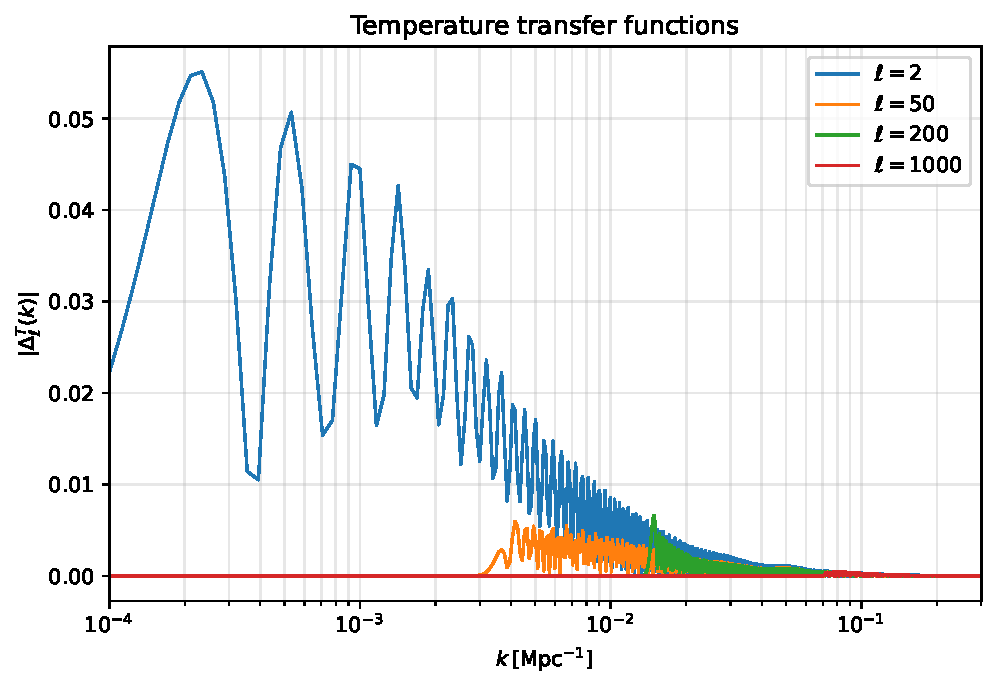
\includegraphics[width=0.95\linewidth]{figures/07_transfer_functions.pdf}
\end{center}

\noindent The figure above is schematic; once you have the source functions for all $k$, the line-of-sight integral in chapter 5 will produce the real $\Delta_\ell(k)$ which you can plot from \texttt{result['Delta\_T']}.

\subsection{Looking ahead}

We now have everything needed for the line-of-sight integral: source-function building blocks per $(k, \tau)$. The remaining work is bookkeeping and numerical efficiency: pick the right grids in $k$ and $\tau$, do the LOS integral for every $\ell$, integrate against the primordial power spectrum. That is chapter 5.
